
% this file is called up by thesis.tex
% content in this file will be fed into the main document

%: ----------------------- introduction file header -----------------------
\chapter{Cross-lingual Document Similarity}\label{ch:multilinguality}

\graphicspath{{multilinguality/figures/}}

% -------------------------------------------------------------
% -- Multilinguality
% -------------------------------------------------------------
% - Mimno et al., 2009. Polylingual topic models.
% - Jagarlamudi & Daume III, 2010. Extracting multilingual topics from unaligned comparable corpora.
% - Boyd-Graber & Resnik, 2010. Holistic sentiment analysis across languages: Multilingual supervised latent Dirichlet allocation.
% - Shi et al., 2016. Detecting common discussion topics across culture from news reader comments. 
% - Hao & Paul, 2018. Learning Multilingual Topics from Incomparable Corpora.
% - Yuan et al., 2018. Multilingual Anchoring: Interactive Topic Modeling and Alignment Across Languages.
% - Yang et al., 2019. A Multilingual Topic Model for Learning Weighted Topic Links Across Corpora with Low Comparability.


As stated in Chapter \ref{ch:hypothesis}, the last of our hypotheses aims to determine whether documents in different languages can be related without having to translate them, by using language agnostic concepts from their main topics (H1.4). In particular, our goal is to find abstractions that capture the content of documents, independently from the language used, in order to draw relations between them. For example, one way of achieving abstraction is by creating multilingual topics from comparable or parallel corpora and relating documents from their topic distributions. A parallel corpora contains sentence-aligned documents (e.g. Europarl\footnote{https://ec.europa.eu/jrc/en/language-technologies/dcep} corpora), and a comparable corpora contains theme-aligned documents (e.g. Wikipedia\footnote{https://www.wikipedia.org/} articles). Other types of abstractions may be obtained using multilingual dictionaries to translate documents in a common language from which they can be related, as shown in Section \ref{sec:multi-topic-alignment}. 

But these approaches based on aligned corpora or document translations require prior knowledge. Connections at document-level (by parallel or comparable corpora) or at word-level (by dictionaries) are necessary to create topic models that represent documents in a common, language-independent space. In this way, the pre-established language relations condition the creation of the topics (supervised method), instead of being inferred from the topics themselves as a posteriori knowledge (non-supervised method). We propose a completely unsupervised way of building cross-lingual topic models that uses sets of cognitive synonyms (\textit{synsets}) to establish relations between language-specific topics once the model is created and does not require parallel or comparable data for training. These models can be used for large-scale multi-lingual document classification and information retrieval tasks.

In Section \ref{sec:synset-space}, we define the language independent conceptual abstractions for topic models. Topics are no longer described by words, but by concepts. They are based on a multilingual knowledge base where nouns, verbs, adjectives and adverbs are grouped into sets of synsets, each expressing a distinct concept. 

In Section \ref{sec:crosslingual-models} and \ref{sec:crosslingual-evaluation}, we create cross-lingual models from synset-based representations of topics and analyze relations between documents described with these models. The analyses were performed from different perspectives. One analysis consists of cross-lingual document classification, while the other one performs cross-lingual information retrieval.

\section{Synset-based Representational Space}
\label{sec:synset-space}

Each topic is annotated with a list of synset \citep{Bond2013} retrieved from WordNet\footnote{https://wordnet.princeton.edu/}\citep{Miller1995WordNet:English} based on its top$n$ words (Fig \ref{fig:density_hash2}). Word by word are queried in WordNet to retrieve its synsets. The final set of synsets for a topic is the union of the synsets from the individual top-words of a topics. Based on empirical evidence from different executions of the algorithm, n=5 is the configuration that offered the best performance in our tests. Let's look at an example to clarify how it works. Given the topics of Table \ref{tb:topics}, the EN-Topic (\textit{"communications systems"}) is annotated with the following synset list: \textit{radio.a.01, radio.v.01, radio.n.03, radio.n.01, radio\_receiver.n.01, equipment.n.01, network.n.02, network.n.04, network.v.01, network.n.05, network.n.01, net.n.06, communication.n.02, communication.n.03, communication.n.01, regulative.s.01}. The list of synset for the ES-Topic (\textit{"sistema de comunicaci\'on"}) is:  \textit{kit.n.02,team.n.01, equipment.n.01, net.n.02, net.n.05, network.n.05, web.n.06, network.n.01, web.n.02, communication.n.02, communication.n.01, announcement.n.02, spectrum.n.02, spectrum.n.01, creep.n.01, ghost.n.01, apparition.n.02, electromagnetic.a.01}. And the list for FR-Topic (\textit{"systeme de communication"}) is:  \textit{access.n.02, approach.n.07, approach.n.02, access.n.06, access.n.03, access.n.05, assault.n.03, bout.n.02, approach.n.01, entree.n.02, entry.n.01, entrance.n.01, entry.n.03, admission.n.01, submission.n.01, introduction.n.01}. The librAIry NLP service\footnote{http://librairy.linkeddata.es/nlp} was used to identify the list of synsets from a topic description based on top words. It includes the Open Multilingual WordNet\footnote{http://compling.hss.ntu.edu.sg/omw/} \citep{Bond2012}.

\begin{figure}[t]\centering
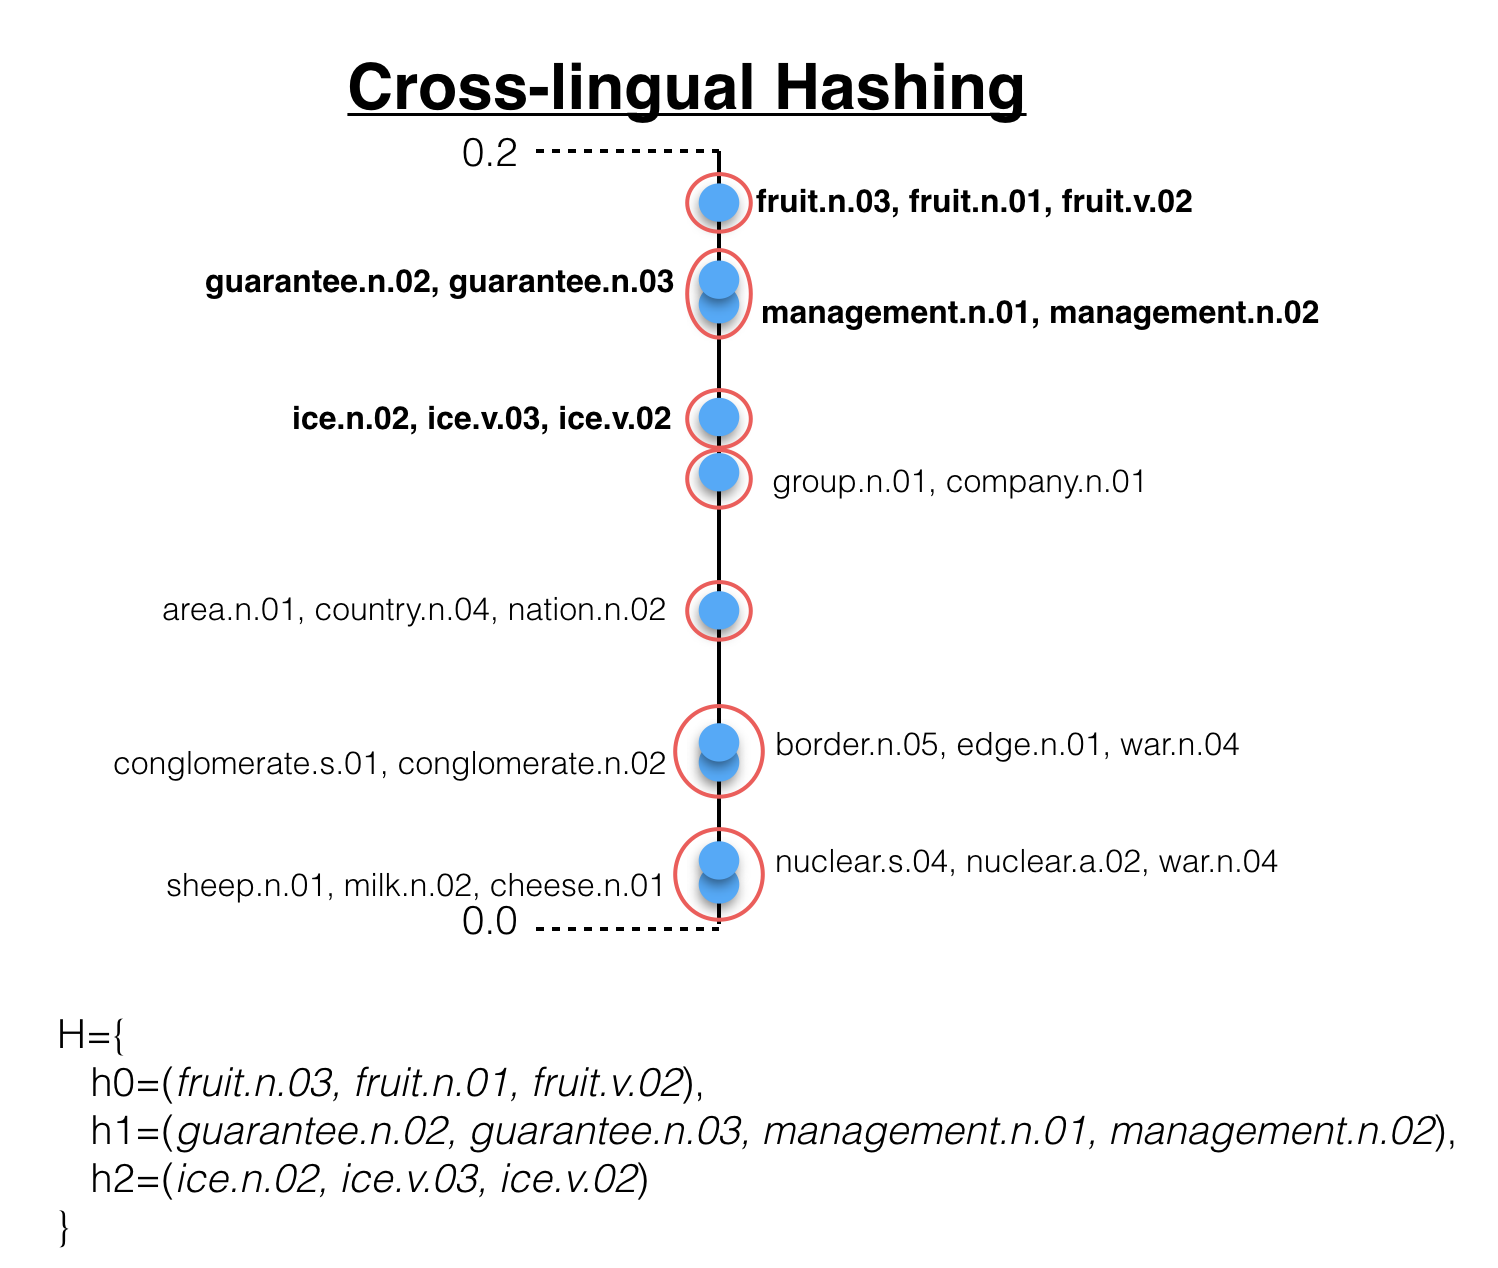
\includegraphics[scale=0.4]{density-hash.png}
\caption{Cross-lingual hash-expression (H) of a document based on WordNet-synset annotations created from the top words of each topic distribution. The most relevant topics are grouped according to their importance in three levels (h0, h1 and h2)}
\label{fig:density_hash2}
\end{figure}

\subsection{Document representation}
Documents (i.e seen as data points in the generated space) are transformed from the original feature space based on mono-lingual topic distributions into a hierarchical-code space, so that similar data points share relevant cross-lingual concepts. Since topic models create latent themes from word co-occurrence statistics in a corpus, a cross-lingual concept specifies the knowledge about the word-word relations it contains for each language. This abstraction can be extended to cover the knowledge derived from sets of topics. The topics are obtained via state-of-the art methods, collapsed Gibbs sampling \citep{Griffiths2004b} for LDA, and hierarchically divided into groups with different degrees of semantic specificity in a document. Documents represented as a weighted mixture of latent topics (per-document topic distributions) are then annotated in these feature spaces with the relation between topics inside each hierarchy level. Regardless of their language, they are then described by cross-lingual concepts (based on WordNet-synset annotations) and hash codes are calculated to summarize their content \citep{Badenes-Olmedo2019}. The hash expression sets a 3-level hierarchy of cross-lingual concepts. Topics with similar presence in a document are grouped together in the same hierarchical level (Fig \ref{fig:density_hash2}). Each level of the hierarchy indicates the importance of the topic according to its distribution. Level 0 describes the topics with the highest score. Level 1 describes the topics with highest score once the first ones have been eliminated, and so on. Documents are described by vectors containing set of topics (i.e. set of synsets), where each dimension means a topic relevance. Given a document $d$ with a topic distribution $q = [t0=0.28, t1=0.05, t2=0.44, t3=0.23]$, the hash expression may be $H_d = {(ts2), (ts0,ts3), (ts1)}$. It means that topic $t2$ described by the synset $ts2$ is the most relevant (i.e 0.44 score), then topics $t0$ and $t3$ described by synsets $ts0$ and $ts3$ (i.e 0.28 and 0.23 scores) and, finally, topic $t1$ described by synset $ts1$ (i.e 0.05).

\begin{figure}[t]\centering
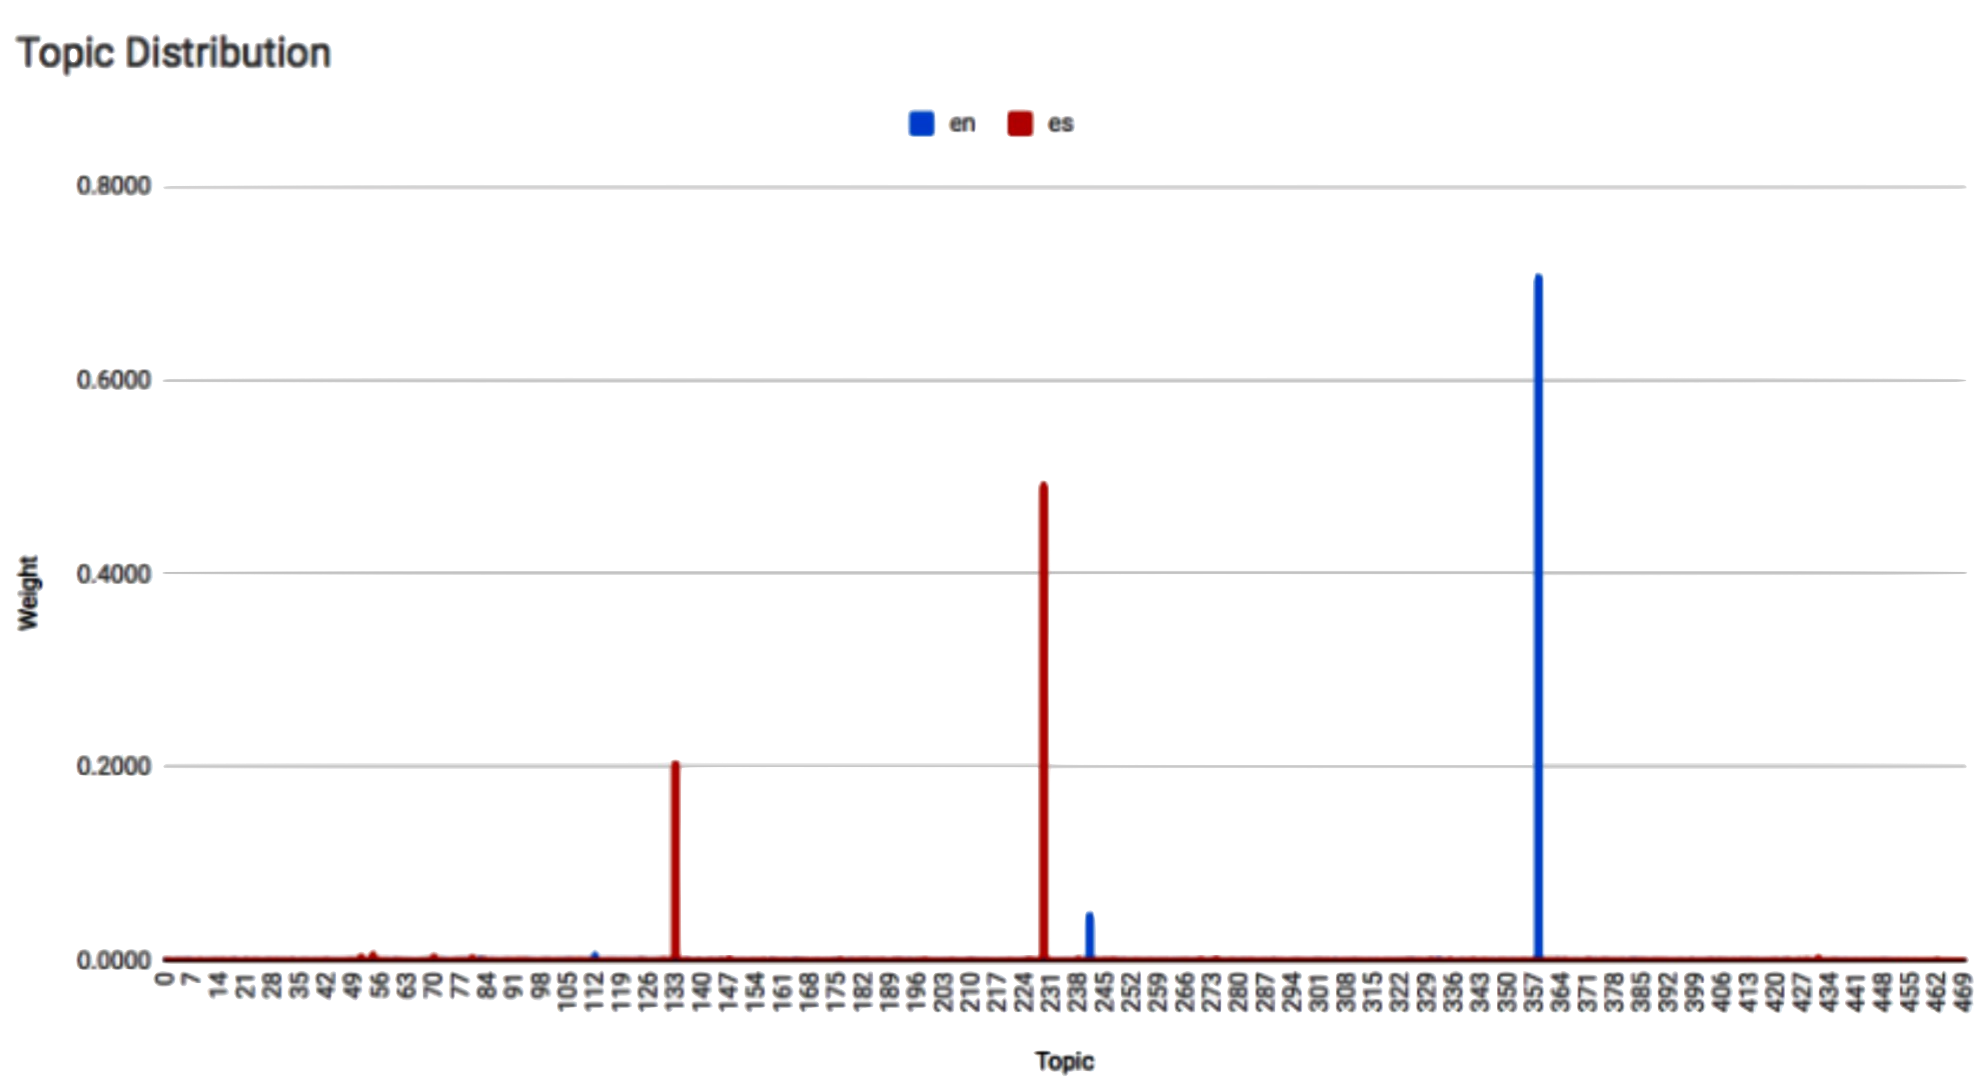
\includegraphics[scale=0.4]{topic-dist.png}
\caption{topic distributions from the same document in English ($h_{EN}=\{(t3062),(t335),(t8278)\}$) and Spanish ($h_{ES}=\{(t335),(t4060),(t5769)\}$).}
\label{fig:topic_distributions}
\end{figure}

\subsection{Similarity metric}
In this workspace based on hierarchical representations of topics we use the distance metric proposed in Section \ref{sec:large-distance-metric} based on the Jaccard coefficient. This metric is mainly used for set-type data \citep{Li2012, Ji2013, Li2010b, Zhao2013} and computes the similarity of sets by looking at the relative size of their intersection (See Eq. \ref{eq:jc}). Thus, it allows us to measure the intersection of cross-lingual topics described by hierarchical hash-sets:

%distance metric formula
\begin{equation}
d_H(H_A,H_B) = \sum\limits_{l=1}^L \Big( d_J(H_A(h_l),H_B(h_l)) \Big) = 
\sum\limits_{l=1}^L \Big( 1 - \frac{H_A(h_l) \cap H_B(h_l)}{H_A(h_l) \cup H_B(h_l)} \Big) 
\label{eq:dh2}
\end{equation}

where $H_A$ and $H_B$ are hash codes, $H_A(h_l)$ and $H_B(h_l)$ are the set of topics up to level $l$ for each hash code $H$,  and $L$ is the maximum hierarchy level. A corner case is $L=T$, where $T$ is the number of topics in the model. 

\section{Cross-lingual Models}
\label{sec:crosslingual-models}

Our approach considers that cross-lingual models can be built from non-parallel or even non-comparable collections of multilingual documents. It first creates a probabilistic topic model for each language separately, and then annotates the topics with cross-lingual labels (Fig \ref{fig:hash_functions2}). In the same way, the topic distribution of documents expressed through weighted vectors are first transformed into hierarchies of topics according to their relevance. And then documents are described by a 3-level hierarchy of cross-lingual concepts.

In order to be able to compare the performance of our unsupervised algorithm with a semi-supervised algorithm (MuPTM-based) it is necessary to use theme-aligned corpora that map topics across languages. We used the JRC-Acquis\footnote{https://ec.europa.eu/jrc/en/language-technologies/jrc-acquis} corpora \citep{Steinberger2006}. It is a collection of legislative texts written in 23 languages, although we only use English, Spanish and French for the tests. Most texts have been manually classified into subject domains according to the EUROVOC\footnote{http://eurovoc.europa.eu/} thesaurus \citep{Eurovoc1995}, which exists in one-to-one translations into approximately twenty languages and distinguishes about 6,000 hierarchically organised descriptors (subject domains). More than 20k documents were used for each language-specific model, a total of 82,140 texts are included in the training-test package, which is publicly available\footnote{http://librairy.linkeddata.es/data/jrc/select?q=*:*} for reuse.

The JRC-Acquis corpus is annotated with EUROVOC categories. These categories are shared among languages and will serve as support for building the topic models. Moreover, the topic independence assumption \citep{Blei2003} of LDA models should be also satisfied, so the categories must first be moved to their base concepts and therefore disjointed categories. The EUROVOC taxonomy has 7,193 concepts/labels from 21 domain areas such as politics, international relations, european union, law, economics, etc. There are 4,904 reciprocal hierarchical relationships (no polyhierarchy) and 6,992 reciprocal associative relationships. Using hierarchical relations, we identified the root concepts from which all other categories derive. The initial 7,193 labels were then reduced to 452 labels, which are independent (topic independence assumption from LDA is satisfied), and can be used to train the topic models. 

\begin{table*}\centering
  \begin{tabular}{l|l|l}
  \hline
      \multicolumn{1}{c}{EN-Topic 3} & \multicolumn{1}{c}{ES-Topic 3} & \multicolumn{1}{c}{FR-Topic 26}  \\
      \multicolumn{1}{c}{\textit{"communications systems"}} & \multicolumn{1}{c}{\textit{"sistema de comunicaci\'on"}} & \multicolumn{1}{c}{\textit{"systeme de communication"}} \\
  \hline
     radio          & equipo                & communications        \\
     equipment      & red                   & reseaux               \\
     network        & comunicaci\'on        & electroniques          \\
     communication  & espectro              & acces                  \\
     regulatory     & electromagn\'etico    & telecommunications     \\
     spectrum       & electr\'onico         & service                \\
     electronic     & reglamentaci\'on      & universel              \\
     access         & banda                 & reglamentaires         \\
     standard       & etsir                 & nationales             \\
     mobile         & compatibilidad        & fourniture             \\
    \bottomrule
  \end{tabular}
\caption{Randonly selected theme-aligned topics described by top 10 words based on EUROVOC annotations from JRC-Acquis dataset}
\label{tb:topics}
\end{table*}

 A pre-processing of the documents was required to clean texts and to build a suitable data set for the model. We assume that terms with high frequency are not specific to a particular topic, so words present in more than 90\% of the corpus are considered stopwords and removed from the model. Also, rare terms that occur infrequently are considered not representative of a single topic since they do not appear enough to infer that it is salient for a topic. Then, words present in less than 0.5\% of the corpus are also removed from the model. Lemmatized expressions of names, verbs and adjectives were used to create the bag-of-words, and documents with less than 100 characters were discarded since LDA has proven to has lower performance with these type of texts \citep{Cheng2014a}. 
 
 Then, we set the number of topics $K=500$ (several configurations were evaluated, but this was the closest to the performance obtained with the supervised model based on categories). We run the Gibbs samplers for 1000 training iterations on LDA from our librAIry framework. The Dirichlet priors $\alpha=0.1$ and $\beta=0.01$ were set following \citep{Hu2014a}. Once the word distributions for each topic is available, the list of synsets related with the top5 words for each topic are identified (this number is set to offer better performance after trying several alternatives). Finally, the 3-level hierarchy of topics per document is replaced by a 3-level hierarchy of synsets. Probabilistic topic models in Spanish\footnote{http://librairy.linkeddata.es/jrc-es-model-unsupervised}, English \footnote{http://librairy.linkeddata.es/jrc-en-model-unsupervised} and French\footnote{http://librairy.linkeddata.es/jrc-fr-model-unsupervised} were created independently without previously establishing any type of alignment between their topics.
 
 In order to compare the performance of this non-supervised approach with approaches based on aligned topics, we need to use a variant of LDA to force the correspondence between the 452 root categories identified in the EUROVOC thesaurus and the latent topics of the model. Thus, LabeledLDA \citep{Ramage2009a}, a supervised version of LDA, was used to perform parameter estimation. Theme-aligned probabilistic topic models in Spanish\footnote{http://librairy.linkeddata.es/jrc-es-model}, English \footnote{http://librairy.linkeddata.es/jrc-en-model} and French\footnote{http://librairy.linkeddata.es/jrc-fr-model} were created sharing the topics but not its definitions (i.e. vocabulary) (see table \ref{tb:topics}).

A simple way of looking at the output quality of the topic models is by simply inspecting top words associated with a particular topic learned during training. A latent topic is semantically coherent if it assigns high probability scores to words that are semantically related \citep{Gliozzo2007, newman-etal-2010-automatic, mimno-etal-2011-optimizing}. It is much easier for humans to judge semantic coherence of cross-lingual topics and their alignment across languages when observing the actual words constituting a topic. These words provide a shallow qualitative representation of the latent topic space, and could be seen as direct and comprehensive word-based summaries of a large document collection.

Samples of cross-lingual topics are provided in Table \ref{tb:topics}. We may consider this visual inspection of the top words associated with each topic as an initial qualitative evaluation, suitable for human judges. Documents present similar topic distributions when projecting their content on topics according to their language as can be seen in fig \ref{fig:topic_distributions}. Since the topic identifiers are not aligned, the graphs appear displaced.

\section{Evaluation}
\label{sec:crosslingual-evaluation}

A way to evaluate our cross-lingual document similarity algorithm is to test how well it performs in practice for different real-life tasks: document classification and information retrieval. Evaluation is done using the B-Cubed metrics \citep{Bagga1998} to estimate the fit between two clusters, the one obtained from a supervised category-based topic alignment algorithm and the one obtained from our unsupervised synset-based topic alignment algorithm. 

% table monolingual JRC
\begin{table}[ht]\centering
\begin{center}
\small
\begin{tabular}{cc|rr||rr||rr}
    \hline
    \multicolumn{8}{c}{\textbf{JRC-Acquis Corpora}} \\
    \hline
    & & \multicolumn{2}{c}{\textbf{en}} &
      \multicolumn{2}{c}{\textbf{es}} &
      \multicolumn{2}{c}{\textbf{fr}} \\
    & & {\textit{cat}} & {\textit{syn}} & {\textit{cat}} & {\textit{syn}} & {\textit{cat}} & {\textit{syn}} \\
    \hline
    \multirow{4}{*}{\textbf{prec}} 
    &{\textit{min}}     &0.01 &0.01 &0.01 &0.01 &0.01 &0.01 \\
    &{\textit{max}}     &1.00 &0.95 &1.00 &0.87 &1.00 &0.87 \\
    &{\textit{mean}}    &\textbf{0.58} &0.48 &\textbf{0.55} &0.48 &\textbf{0.55} &0.41 \\
    &{\textit{dev}}     &0.27 &0.23 &0.27 &0.22 &0.26 &0.20 \\
    \hline
    \multirow{4}{*}{\textbf{rec}} 
    &{\textit{min}}     &0.01 &0.03 &0.01 &0.04 &0.01 &0.05 \\
    &{\textit{max}}     &0.96 &1.00 &0.93 &1.00 &0.95 &1.00 \\
    &{\textit{mean}}    &0.39 &\textbf{0.52} &0.36 &\textbf{0.49} &0.42 &\textbf{0.51} \\
    &{\textit{dev}}     &0.24 &0.20 &0.23 &0.20 &0.23 &0.23 \\
    \hline
    \multirow{4}{*}{\textbf{f1}} 
    &{\textit{min}}     &0.02 &0.03 &0.01 &0.02 &0.02 &0.03 \\
    &{\textit{max}}     &0.70 &0.75 &0.70 &0.71 &0.70 &0.73 \\
    &{\textit{mean}}    &0.35 &\textbf{0.42} &0.32 &\textbf{0.41} &0.37 &\textbf{0.39} \\
    &{\textit{dev}}     &0.16 &0.15 &0.15 &0.15 &0.17 &0.17 \\
\end{tabular}
\end{center}
\caption{Document classification performance (precision-'prec', recall-'rec' and fMeasure-'f1') of the categories-based (\textit{cat}) and synset-based (\textit{syn}) topic alignment algorithms in monolingual document collections (en, es, fr)}
\label{tb:mono-class}
\end{table}


Let $CL_i$ be the cluster that document $t_i$ gets clustered in, and $G_i$ its correct cluster from the ground truth. The B-Cubed metric then calculates $precision=\frac{|CL_i \cap G_i|}{|CL_i|}$ and $recall=\frac{|CL_i \cap G_i|}{|G_i|}$. The total precision and recall of the clustering are taken as the average of the precision and recall scores over all documents. Results are also presented in terms of the $F_1$ measure to balance between precision and recall: $F_1=\frac{2 \cdot precision \cdot recall}{precision + recall}$. The aim is to measure the performance of the algorithm taking into account documents with manual category assignments.

\subsection{Cross-lingual Document Classification}
A random group of 1k documents from the JRC-Acquis corpora, which have not been used to train the models, is considered for evaluation as they are manually tagged with EUROVOC categories. For each document, the cluster to which it belongs is identified from its categories. This cluster is then compared (B-Cubed metrics) with the one obtained from the labels generated from its most representative topics (\textit{cat}) and with the one obtained from the labels generated with the WordNet-Synsets of those topics (\textit{syn}). Algorithm performance is evaluated in monolingual, bilingual, and multilingual document collections (tables \ref{tb:mono-class} and \ref{tb:multi-class} ) .

% table multi-lingual JRC
\begin{table}[ht]\centering
\begin{center}
\small
\begin{tabular}{cc|rr||rr||rr||rr}
    \hline
    \multicolumn{10}{c}{\textbf{JRC-Acquis Corpora}} \\
    \hline
    & & \multicolumn{2}{c}{\textbf{en-es}} &
      \multicolumn{2}{c}{\textbf{en-fr}} &
      \multicolumn{2}{c}{\textbf{es-fr}} &
      \multicolumn{2}{c}{\textbf{en-es-fr}} \\
    & & {\textit{cat}} & {\textit{syn}} & {\textit{cat}} & {\textit{syn}} & {\textit{cat}} & {\textit{syn}} & {\textit{cat}} & {\textit{syn}} \\
    \hline
    \multirow{4}{*}{\textbf{prec}} 
    &{\textit{min}}     &0.01 &0.01 &0.01 &0.01 &0.01 &0.01 &0.02 &0.02\\
    &{\textit{max}}     &1.00 &0.97 &1.00 &0.98 &1.00 &0.97 &1.00 &0.98\\
    &{\textit{mean}}    &\textbf{0.62} &0.55 &\textbf{0.62} &0.56 &\textbf{0.61} &0.56 &\textbf{0.59} &0.52\\
    &{\textit{dev}}     &0.26 &0.23 &0.25 &0.23 &0.26 &0.23 &0.26 &0.23\\
    \hline
    \multirow{4}{*}{\textbf{rec}} 
    &{\textit{min}}     &0.01 &0.09 &0.00 &0.06 &0.01 &0.07 &0.01 &0.07\\
    &{\textit{max}}     &1.00 &1.00 &0.94 &0.97 &0.91 &0.93 &0.86 &0.93\\
    &{\textit{mean}}    &0.33 &\textbf{0.57} &0.36 &\textbf{0.50} &0.30 &\textbf{0.40} &0.25 &\textbf{0.39}\\
    &{\textit{dev}}     &0.16 &0.23 &0.17 &0.19 &0.13 &0.13 &0.13 &0.15\\
    \hline
    \multirow{4}{*}{\textbf{f1}} 
    &{\textit{min}}     &0.02 &0.02 &0.01 &0.02 &0.02 &0.02 &0.02 &0.05\\
    &{\textit{max}}     &0.75 &0.81 &0.76 &0.81 &0.68 &0.72 &0.62 &0.66\\
    &{\textit{mean}}    &0.36 &\textbf{0.49} &0.38 &\textbf{0.47} &0.35 &\textbf{0.41} &0.30 &\textbf{0.38}\\
    &{\textit{dev}}     &0.16 &0.18 &0.15 &0.18 &0.14 &0.14 &0.11 &0.12\\
\end{tabular}
\end{center}
\caption{Document classification performance (precision-'prec', recall-'rec' and fMeasure-'f1') of the categories-based (\textit{cat}) and synset-based (\textit{syn}) topic alignment algorithms in multi-lingual document collections (en-es, en-fr, es-fr, en-es-fr)}
\label{tb:multi-class}
\end{table}

The results show a higher performance of the semi-supervised algorithm (categories-based topic alignment) in terms of precision, and of the unsupervised algorithm (synset-based topic alignment) in terms of coverage. The cause lies in the set of synonyms generated by WordNet, being able to share the same synset for two different topics. From a more general point of view (fMeasure), the benefit obtained by the increase in coverage (recall) is greater than by the loss of accuracy (precision).


\subsection{Cross-lingual Information Retrieval}
Given a set of documents and a text, the task is to rank the documents according to their relevance to the query text regardless of the language used. The JRC-Acquis corpus is used because by having texts tagged with EUROVOC categories we can build a ground-truth set grouping the documents that share the same codes as those used in the query document. A collection of 1k randomly selected documents (monolingual, bi-lingual and multi-lingual) are annotated by the category-based and synset-based topic alignment algorithms. Then, we randomly take articles to search in D for documents that share the same categories than the query document (i.e  the ground-truth set). Next, the query text is used to search in D for similar documents using category-based annotations and synset-based annotations. We evaluate the performance of the algorithms in terms of precision@3, precision@5 and precision@10 (tables \ref{tb:mono-ir} and \ref{tb:multi-ir} ) .

% table monolingual TED
\begin{table}[ht]\centering
\begin{center}
\small
\begin{tabular}{cc|rr||rr||rr}
    \hline
    \multicolumn{8}{c}{\textbf{JRC-Acquis Corpora}} \\
    \hline
    & & \multicolumn{2}{c}{\textbf{en}} &
      \multicolumn{2}{c}{\textbf{es}} &
      \multicolumn{2}{c}{\textbf{fr}} \\
    & & {\textit{cat}} & {\textit{syn}} & {\textit{cat}} & {\textit{syn}} & {\textit{cat}} & {\textit{syn}} \\
    \hline
    \multirow{2}{*}{\textbf{p@3}} 
    &{\textit{mean}}    &\textbf{0.84} &0.83 &\textbf{0.81} &0.78 &\textbf{0.83} &0.74 \\
    &{\textit{dev}}     &0.26 &0.26 &0.27 &0.29 &0.26 &0.32 \\
    \hline
    \multirow{2}{*}{\textbf{p@5}} 
    &{\textit{mean}}    &\textbf{0.82} &0.80 &\textbf{0.79} &0.75 &\textbf{0.80} &0.72 \\
    &{\textit{dev}}     &0.25 &0.25 &0.25 &0.27 &0.25 &0.29 \\
    \hline
    \multirow{2}{*}{\textbf{p@10}} 
    &{\textit{mean}}    &\textbf{0.77} &0.76 &\textbf{0.75} &0.73 &\textbf{0.77} &0.68 \\
    &{\textit{dev}}     &0.23 &0.25 &0.25 &0.27 &0.24 &0.27 \\
\end{tabular}
\end{center}
\caption{Information retrieval performance (precision@3, precision@5 and precision@10) of the categories-based (\textit{cat}) and synset-based (\textit{syn}) topic alignment algorithms in monolingual document collections (en, es, fr)}
\label{tb:mono-ir}
\end{table}

% table multi-lingual TED
\begin{table}[ht]\centering
\begin{center}
\small
\begin{tabular}{cc|rr||rr||rr||rr}
    \hline
    \multicolumn{10}{c}{\textbf{JRC-Acquis Corpora}} \\
    \hline
    & & \multicolumn{2}{c}{\textbf{en-es}} &
      \multicolumn{2}{c}{\textbf{en-fr}} &
      \multicolumn{2}{c}{\textbf{es-fr}} &
      \multicolumn{2}{c}{\textbf{en-es-fr}} \\
    & & {\textit{cat}} & {\textit{syn}} & {\textit{cat}} & {\textit{syn}} & {\textit{cat}} & {\textit{syn}} & {\textit{cat}} & {\textit{syn}} \\
    \hline
    \multirow{2}{*}{\textbf{p@3}} 
    &{\textit{mean}}    &\textbf{0.84} &0.79 &\textbf{0.86} &0.77 &\textbf{0.85} &0.78 &\textbf{0.85} &0.75\\
    &{\textit{dev}}     &0.25 &0.28 &0.23 &0.28 &0.25 &0.29 &0.24 &0.31\\
    \hline
    \multirow{2}{*}{\textbf{p@5}} 
    &{\textit{mean}}    &\textbf{0.82} &0.76 &\textbf{0.84} &0.75 &\textbf{0.82} &0.76 &\textbf{0.81} &0.72\\
    &{\textit{dev}}     &0.24 &0.26 &0.23 &0.27 &0.23 &0.27 &0.23 &0.28\\
    \hline
    \multirow{2}{*}{\textbf{p@10}} 
    &{\textit{mean}}    &\textbf{0.78} &0.73 &\textbf{0.80} &0.70 &\textbf{0.77} &0.72 &\textbf{0.76} &0.67\\
    &{\textit{dev}}     &0.22 &0.24 &0.22 &0.24 &0.23 &0.26 &0.23 &0.26\\
\end{tabular}
\end{center}
\caption{Information retrieval performance (precision@3, precision@5 and precision@10) of the categories-based (\textit{cat}) and synset-based (\textit{syn}) topic alignment algorithms in multi-lingual document collections (en-es, en-fr, es-fr, en-es-fr)}
\label{tb:multi-ir}
\end{table}

Although the precision values are lower than those obtained by semi-supervised approximation, they are sufficiently promising (around 0.75) to think that introducing improvements in the lemmatization process would increase the quality of the WordNet-synset annotations derived from the most representative words of each topic (precision values close to 0.8 in the English corpus).

\section{Summary}
\label{sec:crosslingual-summary}

In this chapter we have described documents based on topic models that create a unique space of representation between different languages. Topics are created independently for each language, and are projected on concepts instead of words. On concept-based representations, documents in different languages coexist together and can be related. This addresses the last research objective of this thesis (R06, \textit{define a transformation of the topic-based annotations to create a unique representational space out of the particularities from each language}). Representations are analyzed in classification and information retrieval tasks on multilingual document collections. As expected, the performance in terms of accuracy is not as good as that of the approach based on prior knowledge (i.e. topics previously aligned by documents annotated with categories). However, in terms of coverage, the performance of the unsupervised approach is much greater than that offered by the semi-supervised approach, to the point of offering better overall performance (i.e f1) in classification tasks. 
In addition, the algorithm has proved to perform close to the semi-supervised algorithm in information retrieval task, which makes us think that the process of topic annotation by set of synonyms should be improved to filter those elements that are not sufficiently representative. 

In order to perform the evaluations, the new representation system was implemented in our libAIry framework. This extension, together with those described in chapters \ref{ch:explainability} and \ref{ch:comparisons}, cover the last technical objective of this thesis (T04, \textit{create a system capable of finding similar documents automatically}). 